

\section{App Development}  \label{androidapp}
In previous section, DNN for hair and clothes segmentation has been reviewed. In this section, proposed solution to the task of intergrating the model into the Android app is demonstrated. Consequently, the implementation of an Android app is rather easy once you have a proper design and well-defined solutions. 
\subsection{Pipeline}
One of the most important use cases of common beauty or augmented reality applications is real-time camera visuality. In case of the thesis, the beauty app has two instance of these use cases: \emph{Hair Camera} and \emph{Clothes Camera}. Indeed, they are addressed as the most intricate work in the app. To clear it up, I proposed a pipeline used for both the two use cases, however the proposed pipeline is so general that can be reused in other applications.  

\vspace{3mm}
\begin{figure} [H]
    \centering
    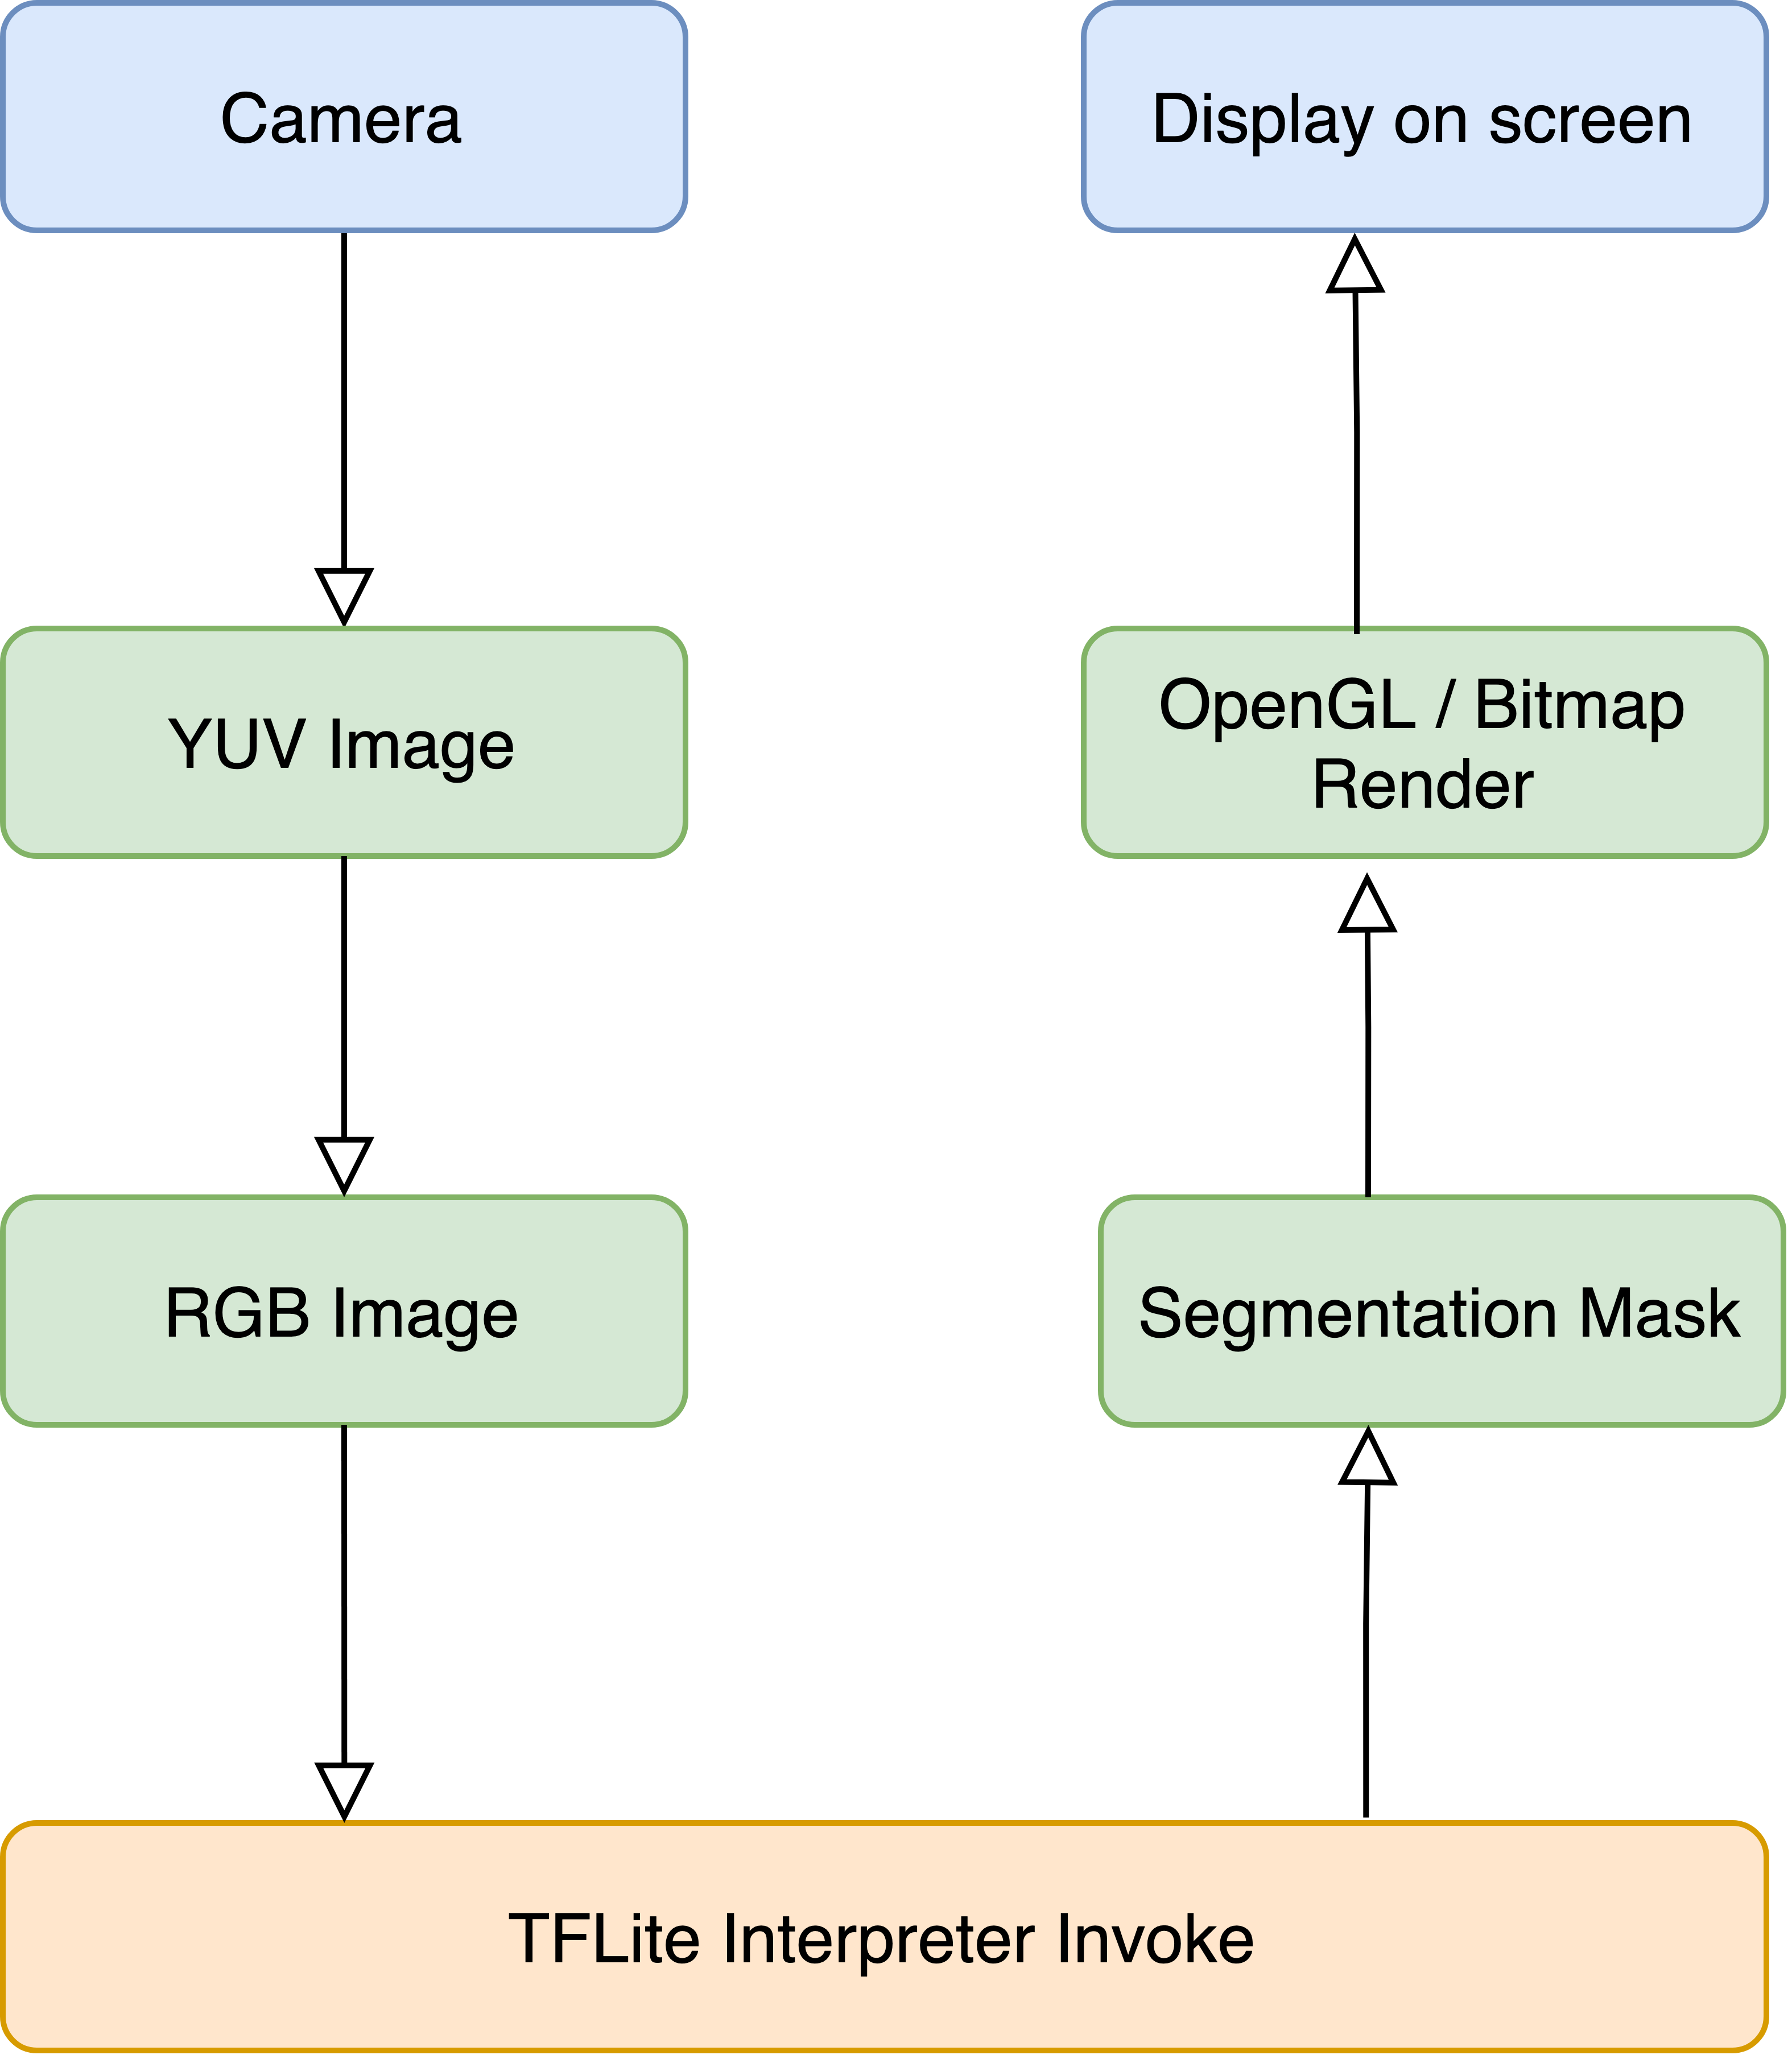
\includegraphics[width=0.6\textwidth]{chapter3/image/apppipeline.png}
    \caption{Pipeline for camera use case}
    \label{fig:my_label}
\end{figure}
 
The pipeline starts with receiving data from hardware, here is the camera lens. CameraX library, which is mention in \textbf{section \ref{sec:camerax}}, supports entire this work.  However, each camera framework outputs image under a different format. For example, if app uses CameraX or Camera2 API, output images are in YUV\_420\_888 format. If app uses Camera API, output images are in NV21 format. After that, the image is converted to a RGB image and represented as byte buffer in order to feed to the model. Subsequently, the TFLite interpreter, which is situated in middle, receives input buffer and outputs the result buffer of the model. The buffer is then preprocessed before being rendered. Finally, the mask is displayed on screen, as a result, the camera view is overlaid with the mask.

 
\subsection{On-device inference}

Making an inference involves taking single or multiple inputs (images, text, video) and pushing them through the many layers of the network. In matters of making on-device predictions, it is vital to have a general understanding of hardware types where the model runs. Almost all smartphones have both CPUs and GPUs. In Android, there are even a few libraries that work with these hardware platforms in order to supply accelerators for deep learning.  \par

Android Neural Networks API (NNAPI) is one of them, which is available for Android 8.1 and above. NNAPI is a machine learning library that supports a wide variety of chipsets, including Snapdragon. There are three options for hardware accelerators, namely GPU, NNAPI, and CPU. Technically, NNAPI is an Android C API designed for executing computationally intensive operations for machine learning on Android devices. NNAPI runtime is a shared library that situated between an app and backend drives, enables NNAPI to run on multiple mobile platforms (Snapdragon, AMD...) \par
 \begin{figure} [H]
     \centering
     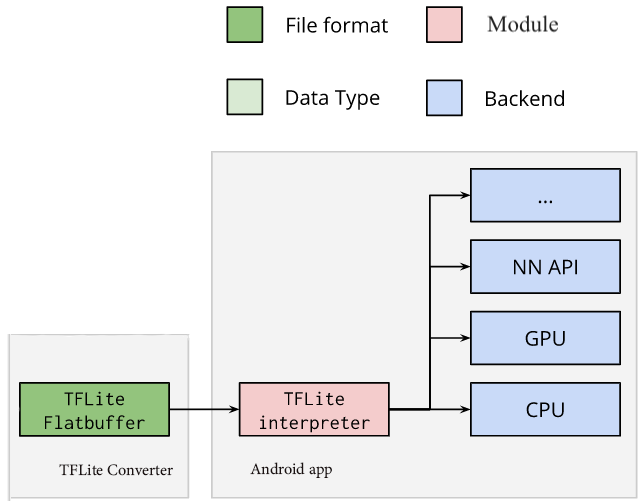
\includegraphics[width=0.7\textwidth]{chapter3/image/client pipleline_edited.png}
     \caption{Workflow of TFLite library for Android}
     \label{fig:my_label}
 \end{figure}
Built upon this, TFLite Interpreter in Android develops both NNAPI delegate and GPU delegate. The GPU delegate is optimized to run 32-bit and 16-bit float-based models where a GPU is available. Although the GPU delegate is well-run and supports more operating systems, I find the NNAPI delegate more effective and battery saving. The following is the code used for preparing input data and run inference with TFLite:\par 
\vspace{5mm}

\begin{lstlisting}[ caption=NNAPI Inference implementation]
// Image pre-processing before feeding into the DNN
private val tfImageProcessor by lazy {
    val cropSize = minOf(bitmapBuffer.width, bitmapBuffer.height)
    ImageProcessor.Builder()
        .add(ResizeWithCropOrPadOp(cropSize, cropSize))
        .add(ResizeOp(
            tfInputSize.height, tfInputSize.width,
            ResizeOp.ResizeMethod.BILINEAR))
        .add(Rot90Op(-imageRotationDegrees / 90))
        .add(NormalizeOp(127.5f, 127.5f))
        .build()
}

// Initialize interpreter with GPU delegate
private val tflite by lazy {
    Interpreter(
        FileUtil.loadMappedFile(this, MODEL_PATH),
        Interpreter.Options().addDelegate(NnApiDelegate())
    )
}

val output =  tflite.run(tfImageProcessor.process(input))
\end{lstlisting}
 
 
 
 
 
 
 
\subsection{Rendering masks}
After semantic information is obtained from the interpreter, segmentation maps are generated. In order to format and display them, two methods of rendering are proposed, namely Bitmap and OpenGL.

\subsubsection{Bitmap}
A bitmap is simply a rectangle of pixels. Each pixel can be set to a given color but exactly what color depends on the type of the pixel. A so-called type of pixels is \emph{ARGB\_8888} where a pixel has four channels (Alpha, Red, Green, Blue) and allocates each eight bits of storage.\par

Bitmap is the first rendering method applied to the app because its well-support in Android API. In fact, Bitmap is a popular 2D graphics class, and Android allows you to use the \emph{Bitmap} class for working with bitmaps. It extends from \emph{Drawable} class which is a general and abstract class for something that can be drawn.  \par


\begin{lstlisting}[caption=Bitmap rendering implementation]
val mask = Bitmap.createScaledBitmap(output, screen.width, screen.height)

overlay.setImageBitmap(
    mask
)
\end{lstlisting}

It would be effective if you do not modify bitmaps too often, because every time you change the content of a bitmap, it is uploaded again as a GPU texture the next time you draw it. As a result, there would have a delay. \par

\subsubsection{OpenGL ES}
OpenGL is a well-used open-source graphic library for rendering 2D and 3D vector graphics on almost all platforms. Android OS is not an exception; it uses a subset of OpenGL’s API called OpenGL for Embedded System (OpenGL ES). OpenGL ES is cross-platform, albeit closed-source. In Android, OpenGL ES is loaded to NDK as a shared library, and SDK wraps it up for ease of implementation.
\par

\begin{figure} [H]
    \centering
    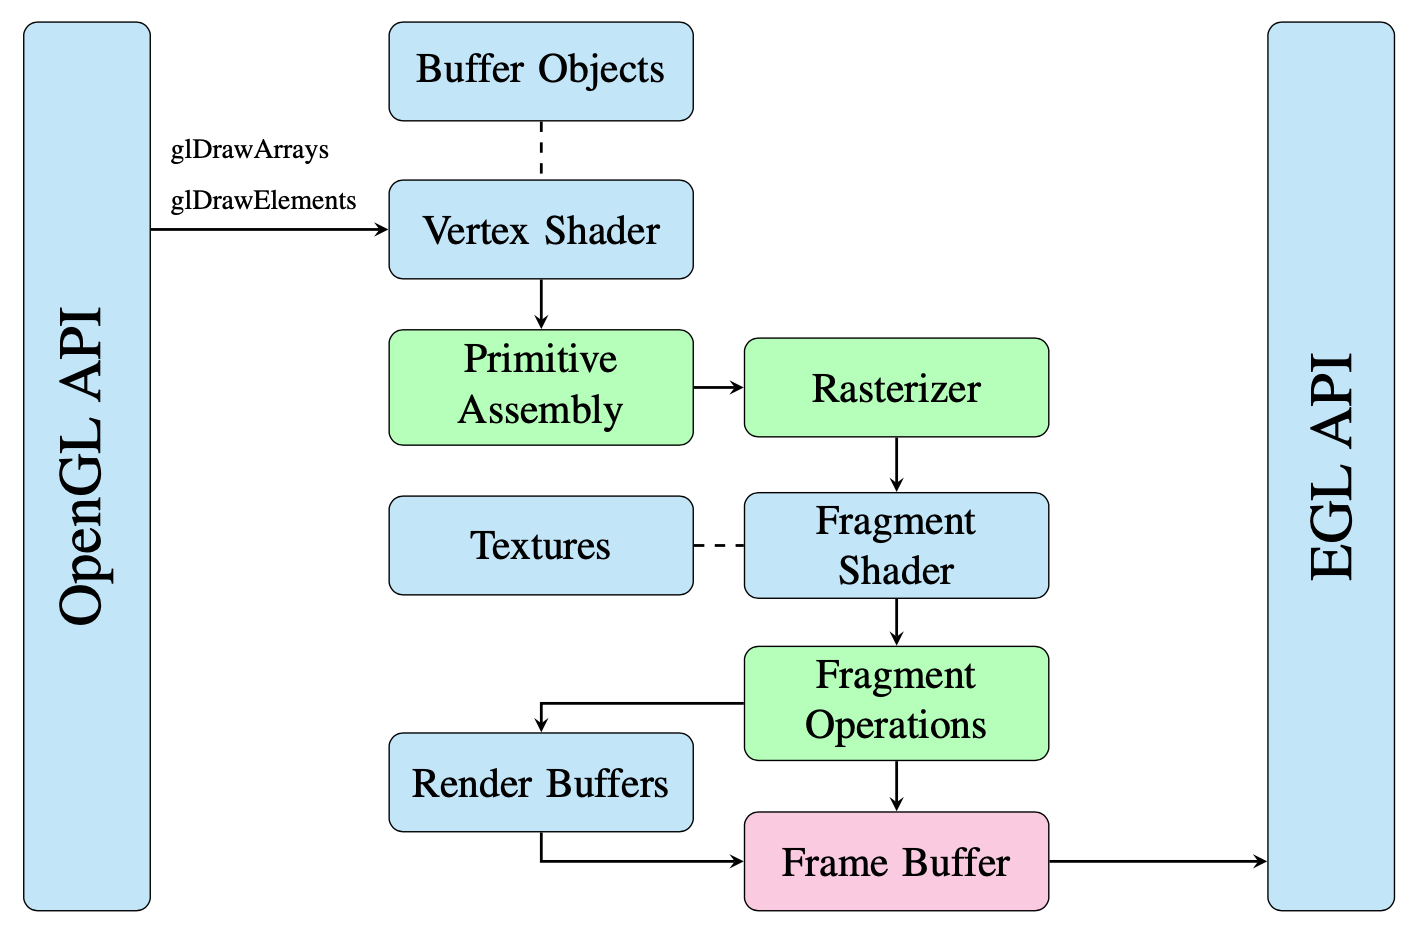
\includegraphics[width=0.7\textwidth]{chapter3/image/openglpipeline.png}
    \caption{OpenGL ES 2.x pipeline. Blue node: You have to set, Green node: You do not have any control, Magenta node: Optional. Source: \cite{openglpipeline}.}
    \label{fig:coordinates}
\end{figure}

The first step in the rendering process is sending the vertices and the texture positions along with the textures, as shown in \textbf{Figure \ref{fig:coordinates}}. To do so, the points that were passed to the renderer first combined into a 1-dimensional array of (x,y,z) values, then uploaded to the vertex shader along with the corresponding texture coordinates of the segmentation mask. These values fall into the range of [−1, 1] in the GLES coordinates, where the point (0, 0) being the middle of the screen. However, the texture coordinates are ranged from [0, 1] where point (0, 0) being the bottom left corner. After the coordinate is uploaded to the vertex shader, the textures are sent to the fragment shader. In the implementation, it was found that it is more efficient to load the whole mask's texture before starting the drawing loop.\par



%We send two different textures to the shader. The segmentation mask which consists of one channel and the color image of the original scene to perform the inpainting in the fragment shader. These textures are sent after the segmentation mask is generated and the hit test is performed by using GLES interface function glTexImage2D. \par

